\documentclass[../fizika.tex]{subfiles}

\begin{document}
    \subsection{Mozgások leírására szolgáló mennyiségek definíciói}

        \subsubsection{Hely, elmozdulás, sebesség és sebességvektor}

            Vegyük fel mindenekelőtt egy egydimenziós \textit{koordinátarendszert}, jelöljük ki az origót és a pozitív $x$ tengelyt. Tegyük fel, hogy a $P$ részecske a $t_2$ időpillanatban az $x_1$ helyen van. Ha a részecske mozog, akkor a $t_2$ időpillanatban új, $x_2$ helyre kerül; azt mondjuk, hogy a részecske \textbf{elmozdulása} $x_2-x_1$. Ezt gyakran a görög $\Delta$ jellel fejezzük ki, ami általában egy mennyiség \textit{megváltozására} utal. Így az 
                \begin{flalign} \tag{1-1} \label{eq:1-1}
                    &\text{Elmozdulás}& &\Delta x = (x_2-x_1)&
                \end{flalign} 
            
            \noindent A $\Delta x$ kifejezés mindig az adott $x$ mennyiség \textit{végső} és \textit{kezdeti} értékének különbségét jelentik. A pozitív $\Delta x$ érték pozitív $x$ irányú, a negatív $-x$ irányú elmozdulást jelöl.

            Az \textbf{átlagsebességet} a pálya mentén megtett teljes út és a megtételéhez szükséges összes idő hányadosa adja.
                \begin{flalign} \tag{1-2} \label{eq:1-2}
                    &\text{Átlagsebesség} &&\text{Átlagsebesség} = \frac{\text{Összes út}}{\text{Összes idő}} &
                \end{flalign} 

            A következőkben az egyenesvonalú mozgás irányának figyelembevételére definiáljuk a $v_{\text{átl}}$ átlagsebesség-vektort.
                \begin{equation*}
                    V_{\text{átl}} = \frac{\text{Elmozdulás}}{\text{Összes idő}}
                \end{equation*}   

                \begin{flalign} \tag{1-3} \label{eq:1-3}
                    &\text{Átlagsebesség Vektor} &&V_{\text{átl}} = \frac{\Delta x}{\Delta t} = \frac{(x_2 - x_1)}{t_2 - t_1} &
                \end{flalign} 

            \noindent Itt $v_{\text{átl}}$ az elmozdulás  előjelétől függően pozitív és negatív is lehet. A pozitív érték azt jelenti, hogy a sebesség a pozitív $x$ irányba mutat, a negatív pedig azt, hogy a sebesség $-x$ irányú.

            \paragraph{A pillanatnyi sebesség}

                A mozgás finomabb részleteire figyelve definiálható a \textit{pillanatnyi sebesség}, ami a mozgást egy adott időpillanatban jellemzi.

                A \eqref{eq:1-3} egyenlet szerint a $t_1, t_2$ időintervallumra az átlagsebesség $v_{\text{átl}} = \Delta x / \Delta t$. Ez az arány a $t_1$ időpillanathoz tartozó $P_1$ pontból a $t_2$ időpillanathoz tartozó $P_2$ végpontig tartó egyenes meredeksége.

                \noindent A $\Delta x / \Delta t$ \textit{arány} (melyet \textit{különbségi hányadosnak} is nevezünk), egy jól meghatározott értékhez, a $t_1$ időpillanathoz tartozó érintő iránytangenséhez tart. Ezt az értéket nevezzük a $t_1$-hez tartozó $v$ \textbf{pillanatnyi sebességnek}.
                    \begin{flalign} \tag{1-4} \label{eq:1-4}
                        &\text{Pillanatnyi sebesség, $v$ (a $t$ időpontban)}& &\eqmathbox{v = \lim_{\Delta t \rightarrow 0} \frac{\Delta x}{\Delta t} = \frac{dx}{dt}}& &&
                    \end{flalign}   
                
                \noindent A $t_1$ időpillanatban a görbe meredeksége pozitív, így a pillanatnyi sebesség is pozitív irányba mutat. A $t_2$ meredekség 0, ami azt jelzi, hogy (ekkor fordul meg a test) a sebesség zérus. A $t_3$ időpontban a meredekség negatív, s ez azt mutatja, hogy a sebesség negatív irányú.

                A \textbf{pillanatnyi sebesség} nagysága megegyezik a \textit{pillanatnyi sebesség abszolút értékével}. 

                A későbbiekben gyakran használjuk majd az előző feladatban kapott általános szabályt, ha $x$ másodfokú függvény (azaz $x = Ct^2$, ahol $C$ állandó), akkor a $v = dx/dt$ derivált $v=C't$ lineáris függvény, ahol $C'$ a $C$-től különböző állandó. Általában fennáll

                    \begin{equation*}
                        \text{Ha } x = Ct^n, \text{ akkor } \frac{dx}{dt} = nCt^{n-1}
                    \end{equation*}

                A $v = v(t)$ függvényábra minden pontban az $x = x(t)$ függvényábra megfelelő pontbeli érintőjének meredekségét adja meg. Negatív $t$ értékek esetén a meredekség is negatív és abszolút értékben annál nagyobb, minél meredekebb a görbe. A $t = 0$ pontban az érintő iránytangense zérus. Pozitív $t$-értékekre pedig pozitívvá válik.

            \subsection{A gyorsulás}

                \noindent Mindenki, aki már vezetett autót, és rálépett a gázra, tudja, hogy mindennapi értelemben a \textit{gyorsulás} a gépkocsi sebességének növekedését jelenti. A fizikában azonban ez a kifejezés általánosabb értelmet nyer és a lassulást is magában foglalja. Ha a $\Delta t = t_2 - t_1$ időtartam alatt egy test pillanatnyi sebessége $\Delta v = v_2 - v_1$-értékkel változik, akkor átlagos gyorsulása definíció szerint
                    \begin{flalign*}
                        &\text{Átlagos gyorsulás} & & \eqmathbox{a_{\text{átl}} = \frac{\Delta v}{\Delta t}} & &&
                    \end{flalign*}
                    
                \noindent A definíció tartalmazza mind a gyorsulást ($a_{\text{átl}}$ pozitív), mind pedig a lassulást ($a_{\text{átl}}$ negatív). A gyorsulás tehát az időegységre eső sebességváltozás. Az SI rendszerben ez $m/s$ osztva másodperccel, azaz $m/s^2$

                A pillanatnyi gyorsulást a pillanatnyi sebesség definíciójához hasonlóan határértékként értelmezhetjük, azaza a pillanatnyi gyorsulás a $\Delta v / \Delta t$ különbségi hányados határértéke, mindőn $\Delta t$ zérushoz tart\footnote[1]{A pillanatnyi gyorsulás második deriváltként is kifejezhető. Mivel $a = \frac{dv}{dt}; a = \frac{d}{dt}(\frac{dx}{dt}) = \frac{d^2x}{dt^2}$}.
                    \begin{flalign*}
                        &\text{Pillanatnyi gyorsulás}& &a = \lim_{\Delta t \rightarrow 0} \frac{\Delta v}{\Delta t} = \frac{dv}{dt} & &&
                    \end{flalign*}

                Szavakban: ,,\textit{a} gyorsulás egyenlő a $\Delta v / \Delta t$ különbségi hányados határértékével, midőn $\Delta t$ zérushoz tart. Ezt a határértéket a sebesség idő szerinti deriváltjának nevezzük és $dv/dt$-vel jelüljük. A $v = v(t)$ grafikonon a $t$ pillanatbeli a gyorsulást $a$ \textit{sebességgrafikon t időpillanathoz tartozó ponthában meghúzott érintő iránytangense} adja meg. A \textit{gyorsulás} szó az esetek többségében \textit{pillanatnyi gyorsulást} jelent, ha kifejezetten $a_{\text{átl}}$-ról kivánunk beszélni, akkor az \textit{átlagos gyorsulás} kifejezést használjuk.

            \subsection{Az egyenesvonalú egyenletesen gyorsuló mozgás kinematikai egyenletei}

                \noindent Azért, hogy a megoldás a legáltalánosabb kezdeti feltételeket kielégítse, feltesszük, hogy $t_0$ kezdeti időpontban adott az $x_0$ kezdeti elmozdulás és $v_0$ kezdeti sebesség. Állandó gyorsulású mozgások esetén az $a$ pillanatnyi gyorsulás megegyezik az $a_{\text{átl}}$ átlagos gyorsulással:
                    \begin{equation*}
                        a = \frac{Delta V}{\Delta t} = \frac{v-v_0}{t-0} = \frac{v-v_0}{t}
                    \end{equation*}

                \noindent amiből átrendezéssel a 
                    \begin{equation} \tag{1-7} \label{eq:1-7}
                        \boxed{v= v_0 + at \;\;\;\;\;\;\;\;\;\;\; \small(\text{állandó }a\text{ esetén})}
                    \end{equation}

                \noindent összefüggéshez jutottunk. Ez a kinematikai feladatok megoldásában rendkívül hasznos un. első kinematikai egyenlet. Legyen a $t_0$ időpontban a kezdősebesség $v_0$. Egy későbbi $t$ időpontban a sebességet a $v = v_0 + at$ egyenes adja, amelynek meredeksége éppen $a = \Delta v/\Delta t$. Az ábrán az egyenes alatti satírozott terület két részre bontható. Az alső, sötétebb téglalap területe $v_0t$, a felső, enyhébben árnyékolt háromszög területe pedig $1/2(v-v_0)t$. Összeadva ezeket a területeket, azt kapjuk, hogy 
                    \begin{equation*}
                        \left[\text{Az egyenes alatti jeles terület}\right] = v_0t+\frac{1}{2}(v-v_0)t= \left(v_0=\frac{v}{2}-\frac{v_0}{2}\right)t
                    \end{equation*}

                    \begin{equation*}
                        \text{Terület} = \left(\frac{v_0+V}{2}t\right)
                    \end{equation*}

                \noindent Az utóbbi formulában a tázójelben éppen a kezdeti és a végsebesség átlaga szerepel, ami a gyorsulás állandósága miatt a $a_{\text{átl}} = \frac{\Delta x}{\Delta t}$ átlagsebességvektorral egyenlő. Felhasználva, hogy $t_0 = 0$ következtében fennáll a $\Delta t = t$-összefüggés, a $\Delta x = x-x_0$, valamint a $\Delta x = a_{\text{átl}}t$ formulák egybevetéséből azt kapjuk, hogy 
                    \begin{equation*} \tag{1-8} \label{eq:1-8}
                        x-x_0= \left[\frac{v_0+v}{2}tableofcontents\right] \;\;\;\;\;\;\;\;\;\;\; (\text{állandó }a\text{ esetén})
                    \end{equation*}

                \noindent Összehasonlítva a két utolsó egyenletet, látható, hogy az $x-x_0$ eredő elmozdulás megegyezik a $v= v(t)$ grafikon alatti területtel. 

                Behelyettesítve a \eqref{eq:1-7} egyenletbe a $v = v_0 + at$ összefüggést, majd az eredményt átrendezve megkapjuk a második kinematikai egyenletnek nevezett formulát:
                    \begin{equation*} \tag{1-9} \label{eq:1-9}
                        \boxed{x=x_0=v_0t+\frac{1}{2}at^2 \;\;\;\;\;\;\;\;\;\;\; (\text{állandó gyorsulás esetén})} 
                    \end{equation*}

                A harmadik szintén nagyon hasznos kinematikai egyenlethez úgy juthatunk el, ha a \eqref{eq:1-7} és \eqref{eq:1-9} egyenletekből elimináljuk az időt. Eredményül a 
                    \begin{equation*} \tag{1-10} \label{eq:1-10}
                        \boxed{v^2=v_0^2+2a(x-x_0) \;\;\;\;\;\;\;\;\;\;\; (\text{állandó }a\text{ esetén})}
                    \end{equation*}

                \noindent formulát kapjuk. \\ Ez utóbbi összefüggés olyan feladatok lehet hasznos, amelyekben az időt nem ismerjük. 

                A kinematikai egyenletek tovább egyszerüsíthetők, ha a koordinátarendszer kezdőpontját ott vesszük fel, ahol a részecske a $t_0 = 0$ időpontban tartózkodik. Ekkor $x_0 = 0$és így két kinematikai egyenlet is egyszerűbbé válik. Természetesen az origó nem mindig választható meg így, amennyiben azonban ez lehetséges, akkor már kezdettől fogva eggyel kevesebb paraméterrel kell dolgoznunk.
                    
                    \noindent\fbox{%
                        \parbox{\linewidth-10pt}{
                            \textbf{\;\;\;\;\;\;\;Az egyenesvonalú egyenletesen gyorsuló mozgás kinematikai egyenletei}

                            \begin{subequations}
                                \begin{empheq}[right={\empheqrbrace =\text{(állandó gyorsulás esetén)}}]{align}
                                    v =& v_0 + at \tag{1-11} \label{1-11}\\
                                    v =& x_0 + v_0t+\frac{1}{2}at^2 \tag{1-12} \label{1-12}\\
                                    v_2 =& v_0^2+2a(x-x_0) \tag{1-13} \label{1-13}
                                \end{empheq}
                            \end{subequations}
                        }
                    }


                További hasznos összefüggéseket kaphatunk az átlagsebesség felhasználásával. Ha a gyorsulás állandó, akkor:
                    \begin{equation*} \tag{1-14} \label{eq:1-14}
                        v_{\text{átl}} = \frac{v_0 + v}{2} 
                    \end{equation*}

                    \begin{equation*} \tag{1-15} \label{eq:1-15}
                        x = x_0 + v_{\text{átl}}t 
                    \end{equation*}

                \noindent A fenti egyenletek - mint már hangsúlyoztuk - csak állandó gyorsulás mellett érvényesek. Ha a gyorsulás időben változik, akkor az integrálszámítás felhasználásával nyerhetünk a sebességre és a helykoordinátára vonatkozó összefüggéseket (\eqref{eq:1-6}, \eqref{eq:1-7} példa). Bár a helykoordináta jelölésére mindig $x$-et használtunk, természetesen hasonló egyenletek írhatók fel az $y$ és $z$ irányú egyenesvonalú mozgásokra is.

                Megjegyzés az előjelekre vonatkozóan: A kinematikai egyenleteket mindig pontosan a \eqref{1-11} - \eqref{eq:1-15} formulákkal megadott alakban kell felírni. 

                A szabadon eső testek gyorsulás-vektora például mindig lefelé mutat. E vektor nagyságát mindig $g$ jelöli.    
                    \begin{flalign*}
                        &\text{A gravitációs gyorsulás a föld felszínén (három értékes jegyre)}& && &g = 9,81 m/s^2&
                    \end{flalign*}

                \noindent Amennyiben a felfelé mutató irányt választjuk pozitívnak, akkor a gravitációs gyorsulás helyére a képletekben $-g$-t kell írni, ha választásunk szerint a lefelé mutató irány a pozitív, akkor a gyorsulás $+g$-vel egyenlő.

            \subsection{A kinematikai egyenletek levezetése differenciálszámítással}

                A 
                    \begin{equation*}
                        v = \frac{dx}{dt}\text{és} \;\;\;\;\;\;\;\;\;\;\;\;\; a = \frac{dv}{dt}
                    \end{equation*}

                \noindent definiáló egyenletek a deriválási művelet megfordításával az integrálással a 
                    \begin{equation*}
                        x = \int vdt \;\;\;\;\;\;\;\;\;\;\;\;\; \text{és} \;\;\;\;\;\;\;\;\;\;\;\;\; v = \int adt
                    \end{equation*}

                \noindent alakban is kifejezhetők. \textit{Állandó gyorsulás} esetén a sebességre 
                    \begin{equation*}
                        v = \int adt = a \int dt = at + C_1
                    \end{equation*}

                \noindent adódik, ahol a $C_1$ integrálási állandó a ,, kezdeti feltételek" figyelembevételével határozható meg, azaz $t = 0$ időpontban a sebesség $v = v_0$. Behelyettesítve a kezdeti feltételt a, 
                    \begin{equation*}
                        v = at + C_1
                    \end{equation*}

                \noindent egyenletbe azt kapjuk, hogy 
                    \begin{equation*}
                        v_0 = (a)\cdot (0) + C_1
                    \end{equation*}

                \noindent ahonnan $C_1 = 0$. Ezzel éppen az első kinematikai egyenlethez jutottunk:
                    \begin{equation*}
                        \boxed{v = v_0 + at \;\;\;\;\;\;\;\;\;\;\; (\text{állandó }a\text{ esetén})}
                    \end{equation*}

                Tovább léphetünk a levezetésben, ha a sebességre kapott kifejezést Behelyettesítjük a helykoordinátát meghatározható integrálba.
                    \begin{equation*}
                        x = \int vdt = \int (v_0 + at)dt
                    \end{equation*}

                    \begin{equation*}
                        x = v_0t + \frac{1}{2}at^2 + C_2
                    \end{equation*} 

                A $C_2$ integrálási állandót ismét a kezdeti feltételekből határozhatjuk meg, azaz abból, hogy $t = 0$ időpontban a mozgó test az $x_0$ helyen van. Ebből azonnal adódik a második kinematikai egyenlet:
                    \begin{equation*}
                        \boxed{x = x_0 + v_0t + \frac{1}{2}at^2 \;\;\;\;\;\;\;\;\;\;\; (\text{állandó gyorsulás esetén})}
                    \end{equation*}

                Az első tag a részecske kezdeti helyzete, azaz a helykoordináta a $t=0$ időpontban, a másik két tag összege pedig éppen a $(0,t)$ időintervallum alábbi eredő elmozdulás.

                    %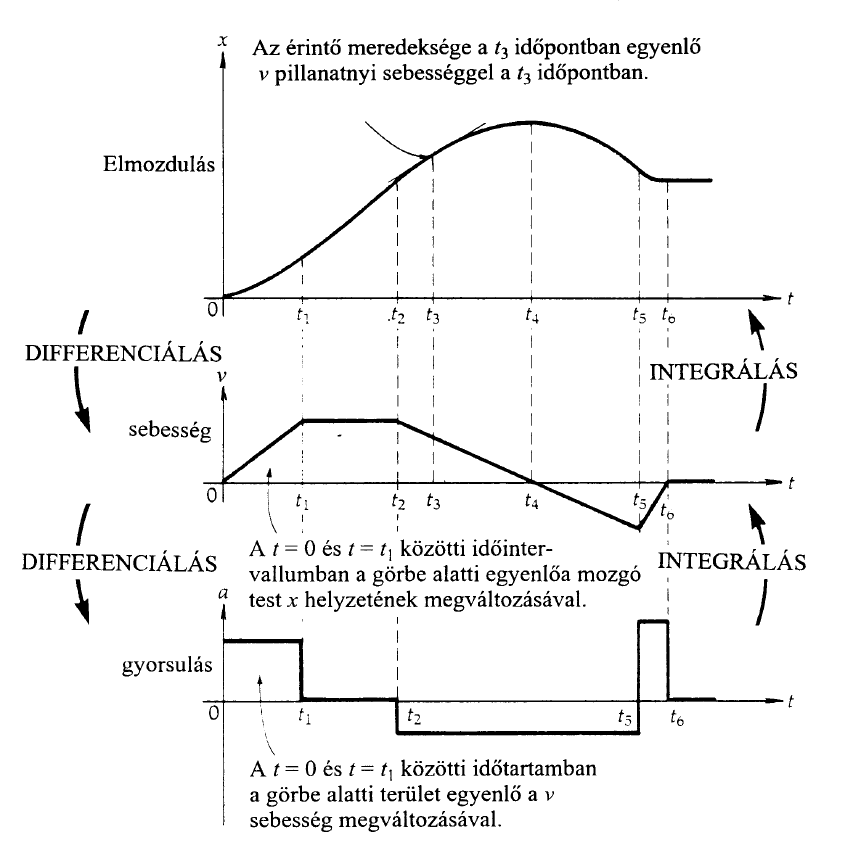
\includegraphics[scale=0.5]{img/1.png}

            \subsection{A dimenzióanalízís}

                \noindent Alapvetően a fizikai egyenletek csak akkor teljesülhetnek, ha a bennük szereplő tagok \textbf{demenziója} azonos. Az egyenletekben csak \textit{azonos dimenziójú tagok szerepelhetnek}.

                \noindent Példaként vizsgáljuk meg a dimenziók egyezése szempontjából a következő kinematikai egyenletet.
                    \begin{equation*}
                        x = x_0 + v_0t + \frac{1}{2}at^2
                    \end{equation*}

                    \begin{flalign}
                        &\text{Dimenziók} & &[L] = [L]+\left[\frac{L}{T}\right][T]+\frac{\left[\frac{L}{T}\right]}{[T]}[T^2]&
                    \end{flalign}

            \subsection{Összefoglalás}

                \begin{multicols}{2}
                    Az egyenesvonalú mozgások leírásakor bevezettük az egydimenziós koordinátarendszert, kijelöltük az origót és az $x$ (vagy $y$, ill $z$) tengely pozitív irányát. Ezután definiáltuk a következő mennyiségeket:
                        \begin{align*}
                            \text{Helyzet:} \;\;\;\; &x\\[1em]
                            \text{Elmozdulás:} \;\;\;\; &\Delta x = x_2 - x_1\\[1em]
                            \text{Átlagsebesség-vektor:} \;\;\;\; &v_a = \frac{\Delta x}{\Delta t} = \frac{(x_2-x_1)}{(t_2 - t_1)}\\[1em]
                            \text{Átlagos gyorsulás:} \;\;\;\; &a_a = \frac{\Delta v}{\Delta t} = \frac{(v_2 - v_1)}{(t_2 - t_1)} 
                        \end{align*}
                    
                    Az így bevezetett mennyiségeknek \textit{nagyságuk} (a mértékegységgel együtt) és pozitív, ill. negatív irányuk van. A $\Delta$ szimbólum a szóban forgó mennyiség megváltozását jelzi. Pl. $\Delta v = v_2 - v_1$. (Figyeljük meg, hogy a változást mindig az adott mennyiség végső és \textit{kezdeti értékeinek különbsége} adja meg!)

                    A kinematikai jellemzők \textit{pillanatnyi értékének} definíciója a következő:
                        \begin{flalign*}
                            &\text{Helyzet:} && x&&& \\[1em]
                            &\text{Sebesség:} & &v = \lim_{\Delta t \rightarrow 0} \frac{\Delta x}{\Delta t} = \frac{dx}{dt}&&&\\[1em]
                            &\text{Gyorsulás:} & & a = \lim_{\Delta t \rightarrow 0} \frac{\Delta x}{\Delta t} = \frac{dx}{dt}&&&
                        \end{flalign*}

                    A megtett út segítségével képzett $ds/dt$ \textit{időderivált} megegyezik a \textit{pillanatnyi sebesség} abszlút értékével. (Az átlagsebességekre vonatkozó analóg állítás nem igaz, hiszen az $s/t$ átlagsebesség többnyire nem egyenlő az átlagsebesség-vektorral.)

                    \noindent A fenti definíciókból néhány, a feladatmegoldásban rendkívül hasznos \textbf{kinematikai egyenlet} vezethető le. Ezek a követketők:

                    \noindent Kinematikai egyenletek:
                        \begin{flalign*}
                            &&&v = v_0 + at&&&\\[1em]
                            &\text{Kinematikai egyenletek}& &v = \lim_{\Delta t \rightarrow 0} \frac{\Delta x}{\Delta t} = \frac{dx}{dt}&&&\\[1em]
                            &&& a = \lim_{\Delta t \rightarrow 0} \frac{\Delta x}{\Delta t} = \frac{dx}{dt}&&&
                        \end{flalign*}
                    
                    \noindent Az állandó gyorsulású mozgások esetén hasznos lehet az alábbi két összefüggés is:
                        \begin{equation*}
                            v_{\text{átl}} = \frac{v_0 + V}{2}
                        \end{equation*}

                        \begin{equation*}
                            x = x_0 + v_{\text{átl}}t
                        \end{equation*}

                    \noindent Ezek az összefüggések csak állandó gyorsulás mellett érvényesek. Ha a gyorsulás az időben változik, akkor a 
                        \begin{equation*}
                            x = \int adt \;\;\;\;\;\;\;\;\;\;\;\;\; \text{és} \;\;\;\;\;\;\;\;\;\;\;\;\; v = \int vdt
                        \end{equation*}

                    \noindent összefüggéseket kell használni.

                    \noindent A formulák egyszerűbbé válnak, ha a koordinátarendszer origóját a $t_0 = 0$ és $x_0 = 0$ feltételeknek megfelelően választjuk meg. Az $y$ és $z$ irányú mozgásra hasonló kinematikai összefüggések írhatók fel. 

                    \noindent A mozgásokkal kapcsolatos feladatok a következő, szabványos módszerrel oldhatók meg:
                        \begin{itemize}
                            \item[(1)] \textit{Megállapítjuk, hogy milyen típusú feladattal van dolgunk.} Ha a gyorsulás állandó, a kinematikai egyenleteket alkalmazzuk. 
                            \item[(2)] \textit{Vázlatot készítünk.} Kijelöljük a kezdőpontot és a pozitív tengelyirányokat, valamint fetüntetjük az alkalmazott jelöléseket. Az ábrára annyi információ kerüljön amennyi világossá teszi a feladatok különböző részei közötti összefüggéseket.
                            \item[(3)] \textit{Csoportosítsuk az ismert adatokat és a keresett mennyiségeket.} Ügyeljünk arra, hogy azonos mértékrendszert használjunk - ha szükséges számítsuk át az adatokat.
                            
                            \noindent Hasonlítsuk össze az adatsort a kinematikai egyenletekben szereplő mennyiségekkel. Ha lehetséges, akkor az origót a $t = 0$ időponthoz tartozóan vagyük fel, hogy $x_0$ ne szerepeljen a kinematikai egyenletekben.
                            \item[(4)] A megoldás után vizsgáljuk meg, hogy a kapott eredménynek van-e ,,értelme". A furcsának tűnő eredmény arra utalhat, hogy hibát követtünk el.
                        \end{itemize}

                    A gravitációs gyorsulás nagyságát $g$-vel jelöljük ($g=9,81 m/s^2$). A föld felszíne közelében $g$ lefelé mutat. Az, hogy előjele pozitív vagy negatív, attól függ, hogy a pozitív irányt felfelé vagy lefelé vesszük fel.

                    A \textit{dimenzióanalízís} az egyenletek mérték szerinti összehasonlításának megállapítására szolgál. Csak azonos mértékegységben kifejezett mennyiségeket szabad összeadni.
                    \end{multicols}

                


\end{document}


$v_{\text{átl}}$ 

\begin{subequations}
    \begin{empheq}[right={\empheqrbrace =f(x)}]{align}
        v =& v_0 + at \tag{1-11} \label{1-11}\\
        v =& x_0 + v_0t+\frac{1}{2}at^2 \tag{1-12} \label{1-12}\\
        v_2 =& v_0^2+2a(x-x_0) \tag{1-13} \label{1-13}
    \end{empheq}
  \end{subequations}